%    Template for seminar reports
% Seminar Current Topics in Computer Vision and Machine Learning
% Summer Semester 2015
% Computer Vision Group, Visual Computing Institute, RWTH Aachen

\documentclass[twoside,a4paper,article]{combine}


% =========================================================================
\usepackage[latin1]{inputenc}
\usepackage{a4}
\usepackage{fancyhdr}   
%\usepackage{german}    % Uncomment this iff you're writing the report in German
\usepackage{makeidx}
\usepackage{color}
\usepackage{t1enc}		% german letters in the "\hyphenation" - command
\usepackage{latexsym}	% math symbols
\usepackage{amssymb}    % AMS symbol fonts for LaTeX.

\usepackage{graphicx}
\usepackage{pslatex}
\usepackage{ifthen}

\usepackage[T1]{fontenc}
\usepackage{pslatex}

\usepackage{psfrag}
\usepackage{subfig}
\usepackage{url}

\usepackage{amsmath}
\usepackage{bm}
\usepackage{float}
% =========================================================================

\setlength{\oddsidemargin}{3.6pt}
\setlength{\evensidemargin}{22.6pt}
\setlength{\textwidth}{426.8pt}
\setlength{\textheight}{654.4pt}
\setlength{\headsep}{18pt}
\setlength{\headheight}{15pt}
\setlength{\topmargin}{-41.7pt}
\setlength{\topskip}{10pt}
\setlength{\footskip}{42pt}

\setlength{\parindent}{0pt}

% =========================================================================

\graphicspath{
	{pictures/}
}

%%%
% We want also subsubsections to be enumerated
%%%
\setcounter{secnumdepth}{3}
\setcounter{tocdepth}{3}

\makeglossary
%\makeindex

% =========================================================================
\begin{document}

% Template for seminar reports
% Seminar Current Topics in Computer Vision and Machine Learning

\begin{titlepage}


\begin{center}
\ 
\vspace{3.5cm}


\textsf
{
Fakult�t f�r Mathematik, Informatik und Naturwissenschaften\\
Institude f�r Informatik II\\
Computer Graphik\\
Jun.Prof. Dr. Angela Yao
}

\rule{\linewidth}{1pt}

\vspace{1.75cm}
\LARGE
\textbf{Lab Report}

\vspace{1.7cm}
\huge
Unsupervised Learning of Video Representations using LSTMs

\vspace{3.0cm}
\Large
Cun Wang\\
\large
Matriculation Number: 362024

\vspace{0.5cm}
July 2017	

\vspace{1.05cm}
\rule{\linewidth}{1pt}

\vspace{0.5cm}
\textsf{\textbf{
\normalsize
\begin{tabular}{ll}
Advisor:  Moritz Wolter\\
\end{tabular}
}}
\end{center}

\end{titlepage}


\begin{abstract}
% +++++++++++++++++++++++++
% Insert your Abstract here
% +++++++++++++++++++++++++
In this lab, Long Short Term Memory (LSTM) networks are used to learn the representation of video sequences. It adpots the Encoder-Decoder
framework. An encoder LSTM is used to map the input sequences to a fixed length representation. Then an decoder LSTM decodes this
representation to reconstruct the input sequences or to predict the future sequences. In order to capture spatiotemporal correlation
better, the convolutional LSTM (ConvLSTM) is applied besides fully-connected LSTM (FC-LSTM).

\end{abstract}

\tableofcontents
\newpage
% =========================================================================

% +++++++++++++++++++++++++
% Insert your Text here
% +++++++++++++++++++++++++

\section{Introduction}
Understanding temporal sequences is important for solving many problems, such as speech recognition, caption generation. Sutksever
\emph{et al.} described a general sequence to sequence learning framework in which a recurrent network is used to encode a sequence into
a fixed representation, and then another recurrent network is used to decode the representation into a sequence \cite{s2s}.
Srivastava \emph{et al.} use the LSTM Encoder-Decoder framework which extends the general framework to learn video representations
\cite{ulvr}.
A sequence of frames are fed in encoder LSTM to generate a representation. This representation is then decoded through another LSTM to 
produce a target sequence. Srivastava \emph{et al.} consider two choices of the target. One choice is to use the inputs as the target 
sequence. The other is to predict the future frames. They also evaluate on two kinds of inputs. One is image patches, the other is the 
high-level "percepts" extracted by applying a convolutional net. In this lab, we only use image patches as the inputs.

LSTM is an important part of Encoder-Decoder framework. LSTM is a specical kind of recurrent neural network, which can capture long-term
temporal dependencies without suffering from the optimization problems such as gradient vanishing. In order to make use of frame structure,
convolutional LSTM introduced in \cite{convlstm} is applied in Encoder-Decoder framework.

\section{Methodology}
\subsection{LSTM architecture}
As mentioned above, Encoder-Decoder framework is composed of LSTMs. We'll introduce vanilla LSTM architecture \cite{odyssey}. A schematic
of the vanilla LSTM block is illustrated in figure \ref{fig:vanilla}. The key to LSTMs is the cell state, which is controlled by three
kinds of gates, namely input gates, forget gates, output gates, adding information to or removing it from the cell state. 
The gates are composed of a sigmoid layer and a pointwise
multiplication operation. The output of sigmoid layer ranges from zero to one, describing how much of each component should be let through.
The forgate gate decides what information is going to be throwed away from the cell state. The input gate decides what information is going
to be stored in the cell state. The output gate decides what is going to output.
\begin{figure}
    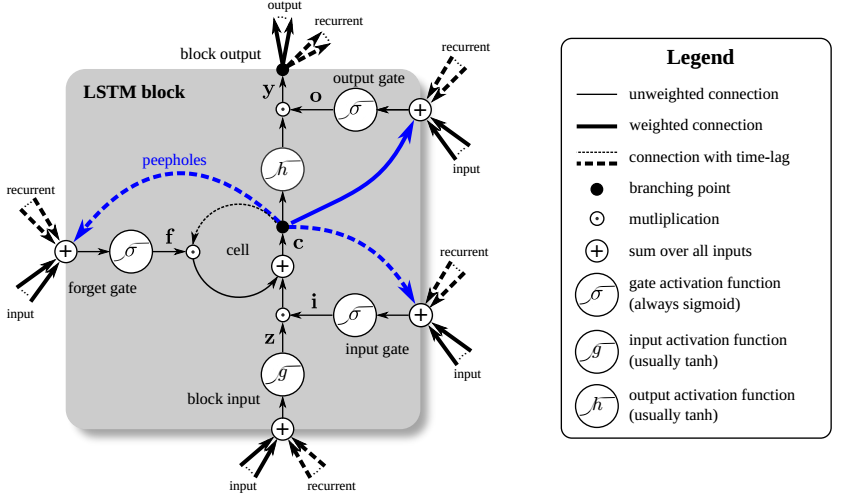
\includegraphics[width=\linewidth]{vanilla}
    \caption{vanilla LSTM block architecture}
    \caption*{Source: \protect\cite{odyssey}}
    \label{fig:vanilla}
\end{figure}

The vector formulas for a vanilla LSTM layer forward pass are given below. $\bm{x}^t$ is the input vector at time t, the $\bm{W}$ are 
rectangular input weight matrices, the $\bm{p}$ are peephole weight vectors and $\bm{b}$ are bias vectors. Using peephole connections, 
the gate layers can look at the cell state. The peephole connections are drawed as the blue lines in figure \ref{fig:vanilla}.
Functions $\sigma$, $g$ and  $h$ are pointwise nonlinear activation functions. $\mathbf{i}$, $\mathbf{f}$, $\mathbf{o}$ are separately
input gate, forget gate, and output gate. The pointwise multiplication of two vectors is denoted with $\odot$:

\begin{align*}
    \mathbf{z}^t &= g(\mathbf{W}_z\mathbf{x}^t + \mathbf{R}_z\mathbf{y}^{t-1} + \mathbf{b}_z) \\
    \mathbf{i}^t &= \sigma(\mathbf{W}_i\mathbf{x}^t + \mathbf{R}_i\mathbf{y}^{t-1} + \mathbf{p}_i\odot\mathbf{c}^{t-1}+ \mathbf{b}_i) \\
    \mathbf{f}^t &= \sigma(\mathbf{W}_f\mathbf{x}^t + \mathbf{R}_f\mathbf{y}^{t-1} + \mathbf{p}_f\odot\mathbf{c}^{t-1}+ \mathbf{b}_f) \\
    \mathbf{c}^t &= \mathbf{i}^t\odot\mathbf{z}^t + \mathbf{f}^t\odot\mathbf{c}^{t-1} \\
    \mathbf{o}^t &= \sigma(\mathbf{W}_o\mathbf{x}^t + \mathbf{R}_o\mathbf{y}^{t-1} + \mathbf{p}_o\odot\mathbf{c}^{t-1}+ \mathbf{b}_o) \\
    \mathbf{y}^t &= \mathbf{o}^t \odot h(\mathbf{c}^t) \\
\end{align*}

As pointed out by Srivastava \emph{et al.}, the key advantage of using LSTM unit over a traditional neuron in an RNN is that the cell state
in an LSTM unit sums activities over time. This is also the reason why LSTM unit don't suffer from gradient vanishing problem. Since
derivatives distribute over sums, the error derivatives don't vanish too quickly as they get sent back into time.

\subsection{Convolutional LSTM}
While traditional multilayer perceptron (MLP) models were to some degree successfully used for image recognition, the appearance of
convolutional neural network (CNN) has made a prominent improvement in many areas such as image recognition, object detection and image
segmentation. The convolutional layer is the core building block of a CNN. With this inspiration, it's straightforward to think of making
the core building block of Encoder-Decoder framework convolutional.
Video frames have spatio information in their structure, which is not captured by FC-LSTM, where full connections are used in
input-to-state and state-to-state transitions. Because of full connections in FC-LSTM, it contains too much redundancy for spatial data.
To make use of spatial information, ConvLSTM is applied in this lab. In the ConvLSTM, the
inputs $\bm{X}_1,...\bm{X}_t$, cell outputs $\bm{C}_1,...\bm{C}_t$, hidden states $\bm{H}_1,...\bm{H}_t$, and gates $i_t,f_t,o_t$ are 3D
tensors whose last two dimensions are spatial dimensions (rows and columns). The ConvLSTM determines the future state of a certain cell
by the inputs and past states of its neighbors, using a convolutional operator in state-to-state and input-to-state transitions. The key
equations are given below, where $\ast$ denotes the convolutional operator and $\odot$ denotes the Hadamard product:

\begin{align*}
    \mathbf{i}_t &= \sigma(\mathbf{W}_{xi} \ast \mathbf{X}_t + 
                        \mathbf{W}_{hi} \ast \mathbf{H}_{t-1} + \mathbf{W}_{ci} \odot \mathbf{C}_{t-1}+ \mathbf{b}_i) \\
    \mathbf{f}_t &= \sigma(\mathbf{W}_{xf} \ast \mathbf{X}_t + 
                        \mathbf{W}_{hf} \ast \mathbf{H}_{t-1} + \mathbf{W}_{cf} \odot \mathbf{C}_{t-1}+ \mathbf{b}_f) \\
    \mathbf{C}_t &= \mathbf{f}_t \odot \mathbf{C}_{t-1} + \mathbf{i}_t \odot tanh(\mathbf{W}_{xc} \ast \mathbf{X}_t +
                        \mathbf{W}_{hc} \ast \mathbf{H}_{t-1} + \mathbf{b}_c) \\
    \mathbf{o}_t &= \sigma(\mathbf{W}_{xo}\ast\mathbf{X}_t + 
                        \mathbf{W}_{ho}\ast\mathbf{H}_{t-1} + \mathbf{W}_{co}\odot\mathbf{C}_{t-1}+ \mathbf{b}_o) \\
    \mathbf{H}_t &= \mathbf{o}_t \odot tanh(\mathbf{C}_t) \\
\end{align*}


\begin{figure}[ht!]
    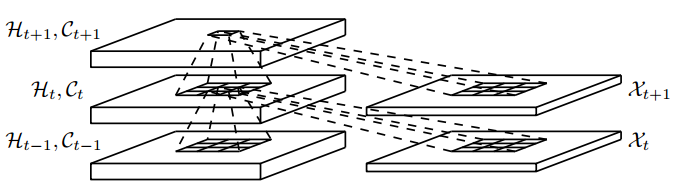
\includegraphics[width=\linewidth]{convlstm}
    \caption{inner structure of convolutional LSTM}
    \caption*{Source: adopted from slides of Kaiming He}
    \label{fig:convlstm}
\end{figure}

\subsection{LSTM autoencoder model}
Autoencoder model is composed of two Recurrent Neural Network, the encoder LSTM and the decoder LSTM, as shown in figure \ref{fig:encoder}.
The input to the model is a sequence of vectors, in our case, video frames. The encoder LSTM runs through these frames to come up with a
representation, which is the state of encoder LSTM atfer the last frame has been read. The decoder LSTM is then expected to reconstruct
target seqence as input sequence based on the representation, which requires that representation contains information about the
appearance of the objects and the background as well as any motion in the video. Srivastava \emph{et al.} point out that it makes
optimization easier when target seqence is reversed compared to input sequence, because the model can look at low range correlation. 

The model has two different design, one in which the decoder LSTM is contioned on the last generated frame and the other in which it is
not. In other word, A conditional decoder receives the last generated output frame as input, described as the dotted boxes in figure 
\ref{fig:autoencoder}.

\begin{figure}[h!]
    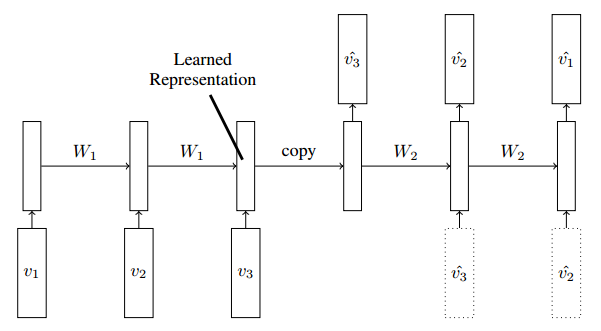
\includegraphics[width=0.8\textwidth]{autoencoder}
    \caption{LSTM Autoencoder Model}
    \caption*{Source: adopted from slides of Kaiming He}
    \label{fig:autoencoder}
\end{figure}

\subsection{LSTM future predictor model}
The future predictor model is similar to the autoencoder model. The only difference is that the decoder of future predictor model
predicates the future frames of a video. The representation generated by encoder need to contain information about which objects are 
present and how they are moving, so that the decoder can predict frames after inputs.
\begin{figure}[ht!]
    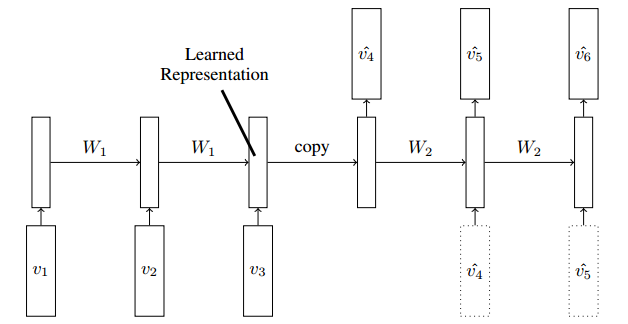
\includegraphics[width=0.8\textwidth]{predictor}
    \caption{LSTM Future Predictor Model}
    \caption*{Source: adopted from slides of Kaiming He}
    \label{fig:predictor}
\end{figure}
\subsection{A composite model}
In the former two section, we talk about the autoencoder model and predictor model separately. Each model suffers from its own
shortcoming. The autoencoder model tends to remember the all the input sequences in its representation when it has high capacity.
The predictor model tends to remember only last few frames, because last few frames have important information to predict upcoming frames.
In order to overcome their shortcomings, the two models can be combined together to create a composite model, as described in figure
\ref{fig:composite}. The composite model has one
encoder for generating the representation from inputs and two decoder, one for reconstructing inputs from encoded representation, the other
for predicting following frames based on the same encoded representation. 
\begin{figure}[ht!]
    \centering
    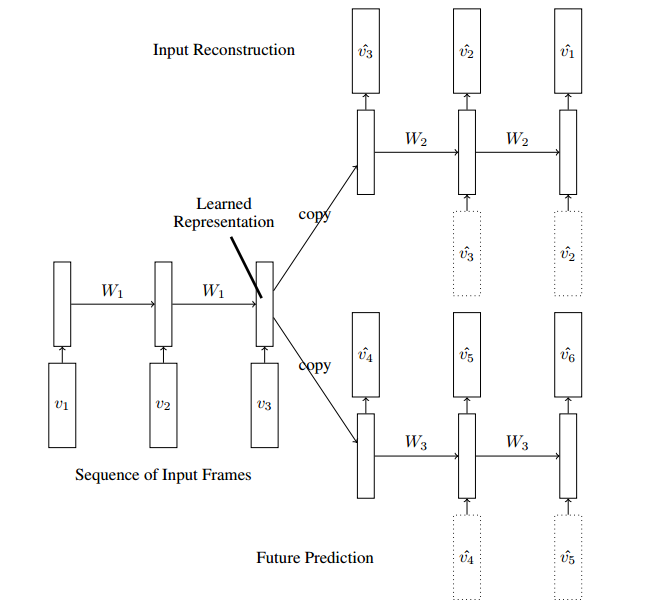
\includegraphics[width=0.8\textwidth]{composite}
    \caption{The Composite Model}
    \caption*{Source: adopted from slides of Kaiming He}
    \label{fig:composite}
\end{figure}

\section{Experiments}
In this lab, experiments are performed to achieve the following objects:

compare the performance of conditional decoder and unconditioned decoder.

check how hyperparameters affect the autoencoder model

compare FC-LSTM and ConvLSTM 

check my implementation of FC-LSTM and ConvLSTM
\subsection{Datasets}
The model is trained on a dataset of moving MNIST digits. Each video is 20 frames long and consist of 2 digits moving inside $64\times64$
patch. The moving digits are chosen randomly from the MNIST dataset and placed initially at random locations inside patch. Each digit is
assigned a velocity with random direction on a unit circle and uniformly random magnitude over a fixed range. The digits bounce off the 
edges of the frame and overlap if they are at the same location.

\subsection{comparision of several complexity}
In this section, we'll compare the perfermance of fully-connected LSTM autoencoder with different LSTM units, which means that they have
different model capability. Models are trained using RMSProp optimizer with initial learning rate at 0.0001. We'll talk more about the
choose of optimizers later.

\begin{table}[h!]
\centering
\begin{tabular}{ c c } 
    \hline
    LSTM units & MSE \\
    \hline
    500 & 0.027440 \\
    1500 & 0.025928 \\
    2500 & 0.019883 \\
    \hline
    \end{tabular}
    \caption{summary of results with different units}
\label{table:units}
\end{table}

\begin{figure}[H]
    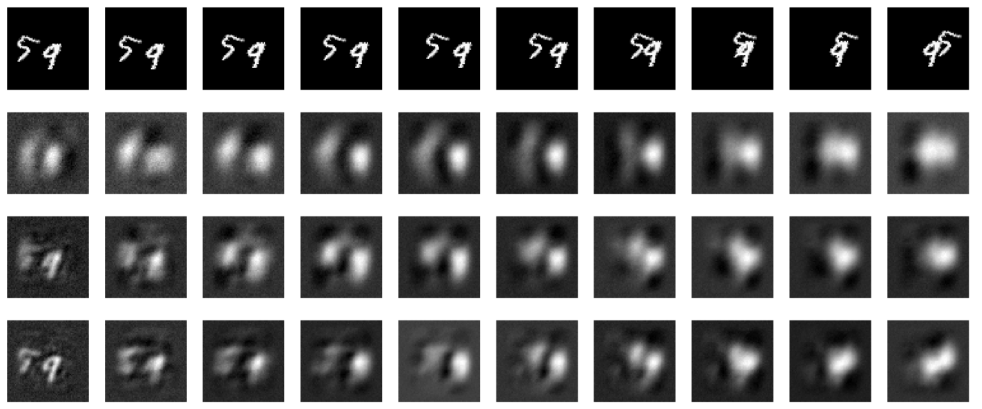
\includegraphics[width=\linewidth]{compare_units}
    \caption{reconstruction of different model capability}
    \label{fig:units}
\end{figure}

\subsection{comparision between fully-connected and convolutional LSTM}
Here we compare the perfermance between autoencoder using fully-connected lstm cells and the one using convolutional lstm cells.
\begin{figure}[H]
    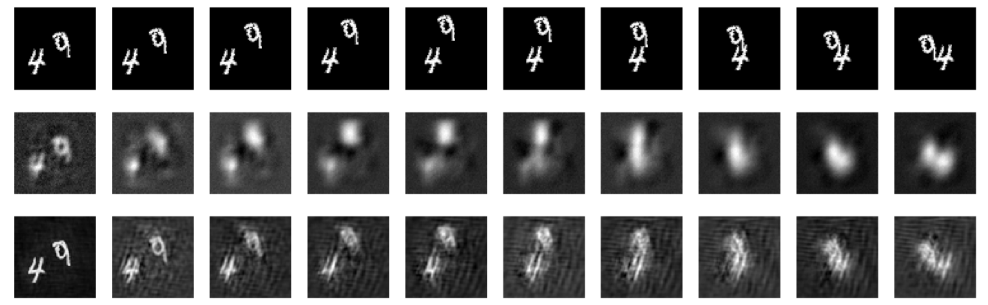
\includegraphics[width=\linewidth]{compare_fc_conv}
    \caption{reconstruction of fc and conv lstm autoencoder}
    \label{fig:fc-conv}
\end{figure}


% =========================================================================
\bibliographystyle{alpha}
\bibliography{lab_report}

% =========================================================================

\end{document}
